% Fig. 1 candidate (illustrative): events -> spiking localiser -> clock and map -> prediction,
% (clock and map). Two-column width (7.16 in = 516 pt).
% Assets: python figures/architecture/make_assets.py.   Build: pdflatex pipeline.tex
\documentclass[tikz,border=1pt]{standalone}
\usepackage[T1]{fontenc}
\usepackage{newtxtext,newtxmath}
\usepackage{graphicx}
\usetikzlibrary{arrows.meta,calc,positioning,fit,backgrounds}

\definecolor{ours}{HTML}{2A78D6}
\definecolor{oursbg}{HTML}{E8F1FC}
\definecolor{onc}{HTML}{E0533F}
\definecolor{offc}{HTML}{3A9BE0}
\definecolor{learn}{HTML}{0F8A5F}
\definecolor{alarm}{HTML}{D03B3B}
\definecolor{ink}{HTML}{0B0B0B}
\definecolor{muted}{HTML}{52514E}
\definecolor{faint}{HTML}{BDBCB6}
\definecolor{mapfill}{HTML}{DCE9FA}

\tikzset{
  font=\footnotesize,
  >={Stealth[length=3.6pt,width=3pt]},
  flow/.style={->, line width=0.7pt, draw=ink},
  lab/.style={font=\scriptsize, text=ink, align=center, inner sep=1pt},
  sub/.style={font=\scriptsize\itshape, text=muted, align=center, inner sep=1pt},
  stage/.style={font=\scriptsize\bfseries, text=muted, anchor=south west, inner sep=1pt},
  group/.style={draw=faint, dashed, line width=0.45pt, rounded corners=3pt, inner xsep=3pt, inner ysep=3pt},
  imgframe/.style={draw=ink, line width=0.5pt, inner sep=0pt},
}

% one feature map drawn in perspective: lower-left corner, width, height, colour
\newcommand{\fmap}[5]{%
  \filldraw[fill=#5, draw=#5!55!black, line width=0.3pt]
    (#1,#2) -- ++(#3,0.45*#3) -- ++(0,#4) -- ++(-#3,-0.45*#3) -- cycle;}
% a stack of n maps, shifted right by dx each
\newcommand{\fstack}[7]{% x, y, width, height, colour, n, dx
  \foreach \k in {1,...,#6} {\fmap{#1+\k*#7-#7}{#2}{#3}{#4}{#5}}}

\begin{document}
\begin{tikzpicture}[x=1mm, y=1mm]
\coordinate (row) at (0,11);       % height of the main left-to-right flow

% ---------------------------------------------------------------- input frame
\node[imgframe, anchor=south west] (ev) at (0,0)
  {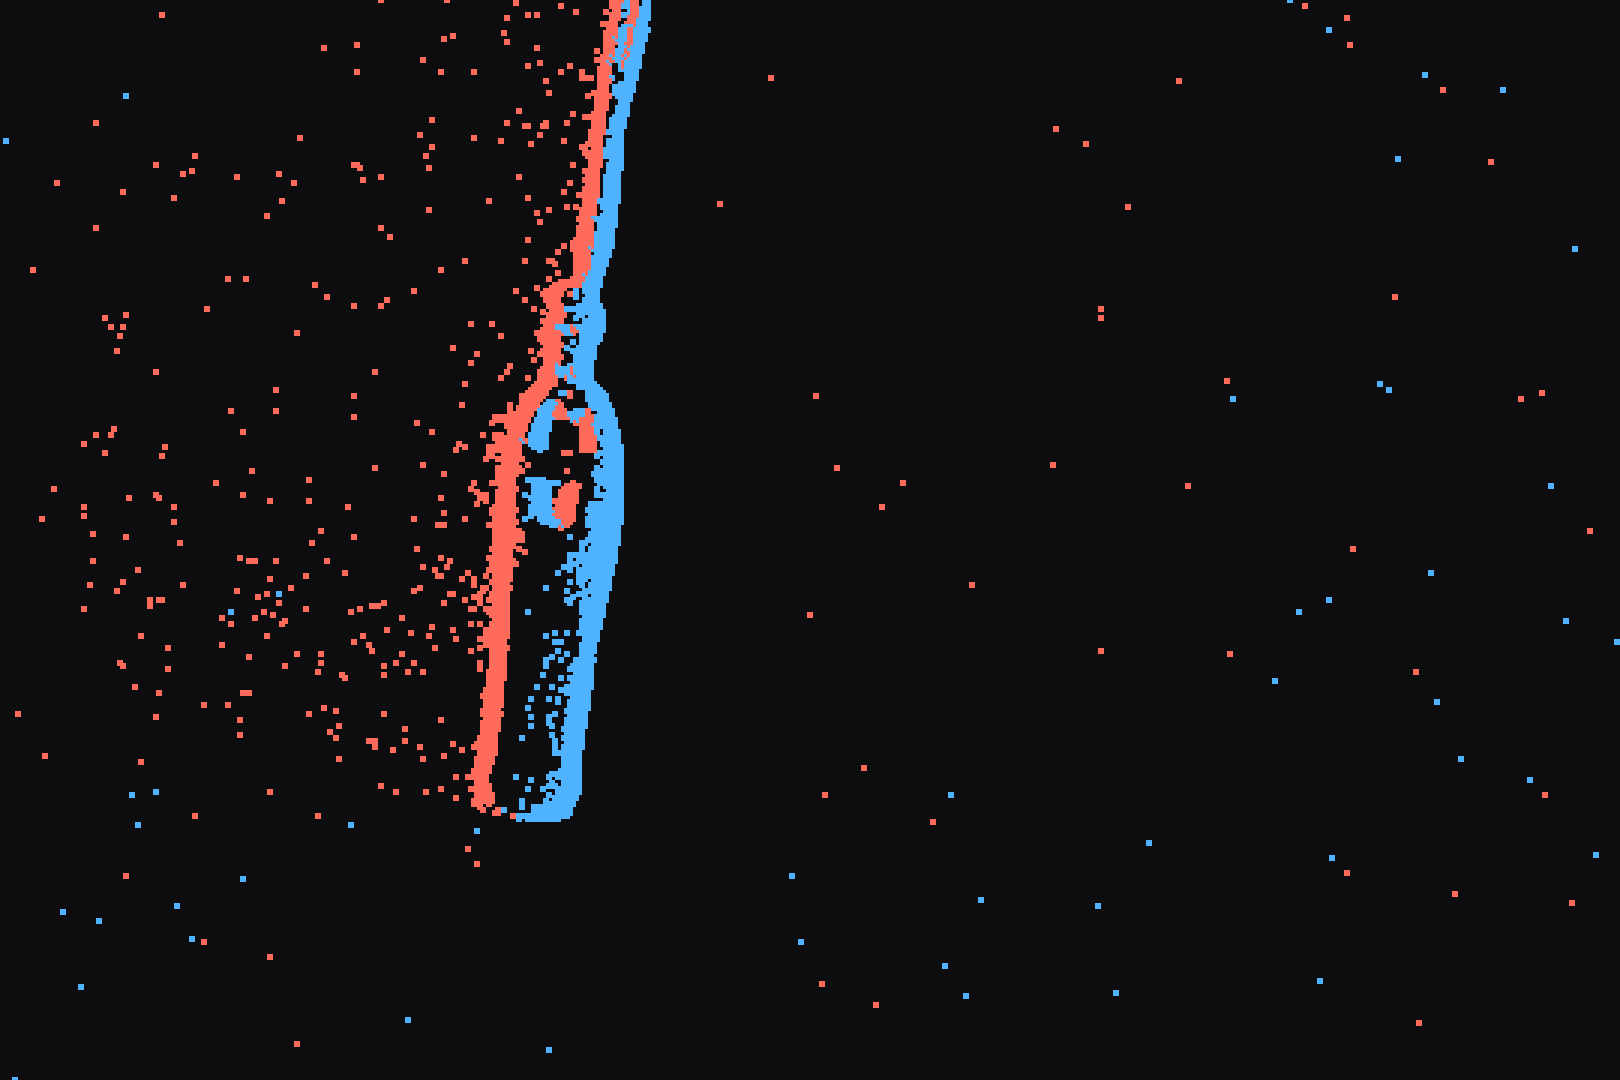
\includegraphics[height=21mm]{assets/event_frame.png}};
\node[sub, anchor=north] at (ev.south) {5\,ms of events\\(ON {\color{onc}$\bullet$}, OFF {\color{offc}$\bullet$})};

% ---------------------------------------------------------------- stage 1: spiking localiser
\begin{scope}[shift={(38,2)}]
  \fstack{0}{0}{7}{15}{ours!30!white}{6}{1.1}
  \fstack{15}{2}{5.2}{11}{ours!45!white}{8}{0.9}
  \draw[ink, line width=0.4pt, fill=white, fill opacity=0.6] (8.44,8.82) -- (10.26,9.64) -- (10.26,12.19) -- (8.44,11.37) -- cycle;
  \draw[muted, line width=0.3pt] (8.44,8.82) -- (15.42,8.35);
  \draw[muted, line width=0.3pt] (10.26,9.64) -- (15.42,8.35);
  \draw[muted, line width=0.3pt] (10.26,12.19) -- (15.42,8.35);
  \draw[muted, line width=0.3pt] (8.44,11.37) -- (15.42,8.35);
  \fill[ink] (15.42,8.35) circle (0.35);
  \draw[muted, line width=0.3pt] (26.50,15.34) -- (31.65,16.80) (26.50,4.34) -- (31.65,3.00);
  \foreach \j in {0,...,6} {\filldraw[fill=ours!60!white, draw=ours!60!black, line width=0.3pt] (32.5,3.0+\j*2.3) circle (0.85);}
  \foreach \j in {0,...,9} {\pgfmathsetmacro{\a}{100*exp(-((\j-3.4)/1.3)^2)}\filldraw[fill=ours!\a!white, draw=ours!70!black, line width=0.25pt] (37.0+\j*0.95,12.2) rectangle ++(0.8,1.6);}
  \node[lab, anchor=east] at (36.6,13.0) {$x$};
  \foreach \j in {0,...,9} {\pgfmathsetmacro{\a}{100*exp(-((\j-4.2)/1.3)^2)}\filldraw[fill=ours!\a!white, draw=ours!70!black, line width=0.25pt] (37.0+\j*0.95,7.2) rectangle ++(0.8,1.6);}
  \node[lab, anchor=east] at (36.6,8.0) {$y$};
  \filldraw[fill=ours, draw=ours!70!black, line width=0.25pt] (38.20,3.20) circle (0.8);
  \node[lab, anchor=west] at (39.2,3.2) {present};
  \node[lab, anchor=north] at (6.5,-1.2) {Conv 1\\[-1pt]{\scriptsize 16 filters}};
  \node[lab, anchor=north] at (21.5,-1.2) {Conv 2\\[-1pt]{\scriptsize 32 filters}};
  \node[lab, anchor=north] at (32.5,-1.2) {Dense\\[-1pt]{\scriptsize 256}\\[-2pt]{\scriptsize neurons}};
  \node[lab, anchor=north] at (42.5,-1.2) {Output};
\end{scope}

% ---------------------------------------------------------------- stage 2: clock, phase cells, map
\begin{scope}[shift={(104,11)}]
  \draw[faint, line width=0.6pt] (0,0) circle (5.2);
  \draw[->, ours, line width=0.9pt] (30:5.2) arc[start angle=30, end angle=95, radius=5.2];
  \draw[muted, line width=0.4pt] (0,0) -- (30:5.2);
  \fill[ink] (30:5.2) circle (0.75);
  \draw[ours, fill=white, line width=0.7pt] (95:5.2) circle (0.75);
  \node[sub] at (0,-1.2) {$\varphi$};
  \node[lab] at (0,-9.3) {clock\\[-1pt]{\scriptsize\itshape adaptive osc.}};
  \begin{scope}[shift={(14,0)}]
    \foreach \a in {0,20,...,340} {
      \pgfmathsetmacro{\d}{min(abs(\a-30), 360-abs(\a-30))}
      \pgfmathsetmacro{\act}{100*exp(-(\d/32)^2)}
      \filldraw[fill=ours!\act!white, draw=ours!60!faint, line width=0.3pt] (\a:5.2) circle (0.8);
    }
    \node[lab] at (0,-9.3) {phase\\[-1pt]cells};
  \end{scope}
  \draw[flow] (5.8,0) -- (7.9,0);
  \begin{scope}[shift={(32,0)}]
    \filldraw[fill=mapfill, draw=ours, line width=0.6pt, rounded corners=1.5pt] (-5,-5) rectangle (5,5);
    \draw[ours, line width=0.9pt] (-3.8,1.8) .. controls (-1.5,-2.2) and (1.5,-2.2) .. (3.8,1.8);
    \node[lab] at (0,-9.3) {map\\[-1pt]{\scriptsize\itshape PES-learned}};
    \node[sub, anchor=south] at (0,5.3) {read at $\varphi{+}\omega h$};
  \end{scope}
  \draw[flow] (20,0) -- (26.6,0);
\end{scope}

% ---------------------------------------------------------------- output frame
\node[imgframe, anchor=south west] (out) at (148.5,0)
  {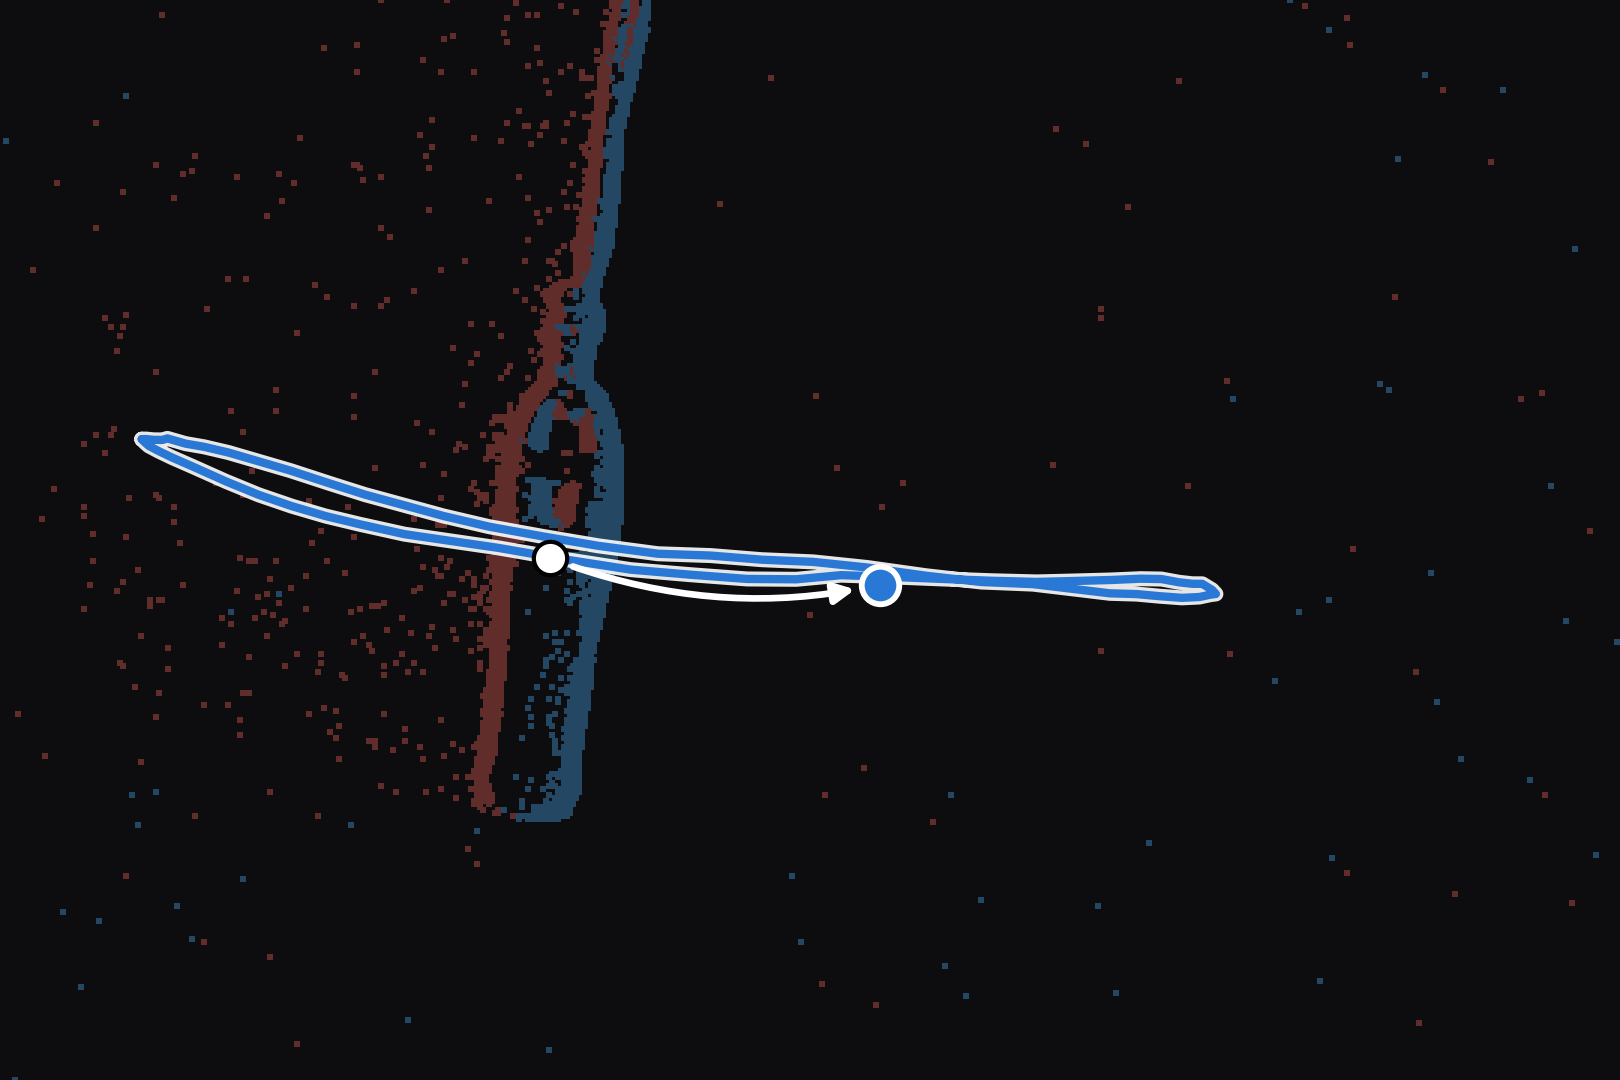
\includegraphics[height=21mm]{assets/prediction_frame.png}};
\node[sub, anchor=north, align=left] at (out.south) {%
  {\color{ours}\textbf{---}} remembered path\\
  $\circ$ $p(t)$\quad {\color{ours}$\bullet$} $\hat{p}(t{+}100\,\mathrm{ms})$};

% ---------------------------------------------------------------- stage boxes and the flow between them
\begin{scope}[on background layer]
  \node[group, fit={(36,-7.5) (85,20)}] (g1) {};
  \node[group, fit={(95.5,-7.5) (142,20)}] (g2) {};
\end{scope}
\node[stage] at (g1.north west) {Stage 1: spiking localiser (LIF neurons)};
\node[stage] at (g2.north west) {Stage 2: trajectory memory};

\draw[flow] (ev.east |- row) -- (g1.west |- row);
\draw[flow] (g1.east |- row) -- node[sub, above] {$p(t)$} (g2.west |- row);
\draw[flow] (g2.east |- row) -- (out.west |- row);

\end{tikzpicture}
\end{document}
